\chapter{Métodos y montaje experimental}\label{cap:modeloneuronal_robot}
\graphicspath{{figs/capitulo_modelo_dinamica_neuronal/}}

\chapterquote{We shall assume. . .\\
	. . . that all cows are spherical.
}{old joke}


En el capítulo anterior, se sentaron los fundamentos, tanto biológicos como conceptuales, que sustentan el entendimiento de la dinámica neuronal global en C. elegans. La disponibilidad de grabaciones neuronales a gran escala en organismos modelo ha transformado profundamente nuestras capacidades para llevar a cabo modelizaciones teóricas de la dinámica de poblaciones neuronales. Los recientes avances en tecnologías de imagen de todo el cerebro para el nematodo C. elegans \cite{kato_global_2015}, han desbloqueado la posibilidad de estudiar de manera integral la relación entre la actividad neuronal y los resultados conductuales. Es crucial destacar que C. elegans se presenta como un modelo excepcional que permite cuantificar la dinámica de poblaciones neuronales, ya que cuenta únicamente con 302 neuronas, cuya conectividad electrofisiológica estereotipada (conectoma) se ha detallado minuciosamente a través de microscopía electrónica de secciones seriadas\cite{cook_whole-animal_2019}.


En este contexto, el propósito de esta sección de la tesis es dilucidar cómo se manifiesta el comportamiento en un robot en el que se ha implementado la dinámica neuronal de C. elegans. Este enfoque nos conduce hacia una comprensión más profunda de cómo el sistema nervioso de C. elegans podría llevar a cabo cálculos y tomar decisiones en respuesta a las señales sensoriales que recibe. De acuerdo a la proposición de Kaplan et al., el sistema nervioso del gusano se comprende de mejor manera como un sistema distribuido y dinámico diseñado para generar un comportamiento adecuado, implicando la mayoría de las interneuronas y neuronas motoras. Esta red distribuida recibe entradas de neuronas sensoriales que actúan para modificar su dinámica con el fin de tomar decisiones. De esta forma, el conectoma funciona como una estructura análoga a la arquitectura de una computadora biológica, que, en conjunto con una dinámica neuronal apropiada, posibilita la emergencia del comportamiento.


En la investigación científica, los modelos y simulaciones juegan un rol esencial, proporcionando herramientas valiosas para validar observaciones y teorías relacionadas con las causas subyacentes de comportamientos específicos. No obstante, es vital reconocer que la modelización o simulación de comportamientos específicos puede derivar en interpretaciones sesgadas si no se considera el organismo en su totalidad. No siempre resulta obvio que una pequeña parte del organismo producirá los mismos resultados al incorporar más componentes del organismo al modelo. Para abordar estas limitaciones, en esta sección de la tesis se introduce un robot impulsado por una simulación que abarca todo el conectoma. Además, se proporciona un marco experimental que ilustra cómo se puede aprovechar la no linealidad para crear un modelo global de la dinámica de las poblaciones neuronales y cómo este enfoque puede aplicarse de manera sencilla a organismos modelo más complejos.


Este capítulo también detalla las metodologías utilizadas para comprender cómo se ensamblan las dinámicas de la red y cómo la estructura de la red, en conjunto con las conexiones sinápticas, generan las dinámicas observadas. Dado que los registros de la dinámica neuronal de todo el cerebro en C. elegans proporcionan datos de alta dimensión (datos de series de tiempo de alrededor de 300 neuronas), se torna esencial extraer información relevante mientras se reduce la dimensionalidad de los datos. Esta sección en su conjunto forma un enfoque holístico y coherente para abordar el problema de la dinámica neuronal en C. elegans y su aplicación a modelos más complejos en la investigación científica.




\section{Modelo de dinámica  neuronal}\label{sec:modelo_dinamica_neuronal}



En el transcurso de la locomoción animal, los organismos se ven inmersos en un continuo flujo de señales sensoriales provenientes de su entorno. Por lo tanto, resulta imperativo que los sistemas nerviosos de estos seres vivos sean capaces de discernir información relevante para la conducta, permitiéndoles generar respuestas adaptativas frente a estos estímulos. La comprensión de cómo los circuitos sensoriomotores procesan estas señales de manera adaptable, considerando factores como el contexto y la experiencia, ha sido objeto de una extensa investigación en las últimas décadas \cite{flavell_dynamic_2022}.

En este contexto, la modelización computacional emerge como una herramienta de gran potencial para investigar y comprender el procesamiento de información en sistemas neuronales. Estos modelos desempeñan un papel central en la desentrañación de los mecanismos subyacentes a la transmisión sináptica, el potencial de acción, la integración dendrítica y, más recientemente, la función de los circuitos neuronales. A pesar de la diversidad de estos modelos en cuanto a su nivel de detalle biológico, que va desde simplificaciones de alto nivel que arrojan luz sobre el comportamiento global de los circuitos, hasta modelos biológicamente detallados que permiten explorar en detalle los mecanismos subyacentes a la función de los circuitos, es importante destacar que los modelos biológicamente detallados a menudo se caracterizan por su intrincación y la inclusión de numerosos parámetros. Sin embargo, a pesar de la abundancia de datos experimentales procedentes del mapeo del conectoma, la cartografía de la actividad funcional y las iniciativas a gran escala relacionadas con el cerebro, la confianza en las predicciones de estos modelos suele verse limitada por su complejidad y la percepción de falta de restricción \cite{gleeson_open_2019}.



En lo que respecta al C. elegans, se han desarrollado modelos en varios niveles de complejidad \cite{gleeson_c302_2018}. Estos abarcan desde modelos de neuronas individuales \cite{kuramochi_computational_2017} y músculos \cite{boyle_caenorhabditis_2008}, hasta subcircuitos especializados en la generación de comportamientos específicos \cite{roberts_stochastic_nodate}. Además, se han modelado procesos corporales como la locomoción \cite{izquierdo_integrated_2015} y se han generado modelos detallados del sistema nervioso y la musculatura \cite{palyanov_towards_2012}. La dinámica neuronal en el cerebro completo ha involucrado una variedad de formalismos matemáticos, incluyendo enfoques discretos (como autómatas celulares, redes booleanas y redes booleanas probabilísticas) y continuos (como redes neuronales celulares, ecuaciones diferenciales ordinarias y ecuaciones diferenciales parciales). Entre los ejemplos de estos modelos se encuentran los sistemas dinámicos y los modelos basados en la máxima entropía, respaldados por inferencia estadística, que incluye métodos bayesianos \cite{randi_measuring_2020}. Cada uno de estos enfoques de modelización presenta diferencias sustanciales en cuanto a los parámetros, el nivel de detalle biofísico y el tratamiento del tiempo y la dinámica temporal, tal como se describe en el \Cref{table:modelos_dinamica}.



Cada modelo se enfrenta al desafío de equilibrar la representación de detalles biofísicos, la concordancia con los datos experimentales y la facilidad de interpretación para los investigadores. Por ejemplo, un modelo biofísico detallado puede abordar explícitamente cada sinapsis, lo que facilita la interpretación, pero puede dificultar la extracción de propiedades específicas de las sinapsis a partir de los datos. Por otro lado, un modelo que emplea una descripción eficaz de la red mediante variables latentes puede resultar más adecuado para guiar a los investigadores en la búsqueda de propiedades abstractas de la red. Los parámetros, ya sean numéricos y representativos de las sinapsis incluidas en el modelo, o conexiones abstractas entre las neuronas, son ejemplos de elementos críticos que influyen en la elección y adquisición de parámetros, lo que da forma a la naturaleza de los diferentes modelos.


\begin{table}[h!]
	\centering
	\caption[Variedad de Modelos para Explorar la Dinámica Neuronal en C. elegans.]{ Variedad de Modelos para Explorar la Dinámica Neuronal en C. elegans.  Los modelos utilizados para investigar la dinámica neuronal en el sistema nervioso del C. elegans varían en formas cruciales. Algunos de estos modelos derivan sus parámetros de la red neuronal a partir del conocimiento a priori del conectoma anatómico y estimaciones biofísicas, mientras que otros ajustan sus parámetros en función de registros de la actividad neuronal. (Adaptado de \protect\cite{randi_measuring_2020}) }
	\begin{tblr}{colspec={X[l,4]X[l,2]X[l,3]X[l,2]X[l,3]X[l,4]},
 			row{odd} = {bg=gray8},
			row{even} = {bg=gray9},
			row{1} = {bg=red3, fg=white, font=\sffamily},
		}
		
Formalismo Matemático	& Referencia & Fuente de Parámetros	 & Detalle	 & Grados de Libertad	& Dinámica temporal\\

Sistemas dinámicos	        &  Kunert et al. \cite{kunert_spatiotemporal_2017} &  A priori a partir del conectoma + estimaciones biofísicas  & Biofísico &  Neuronas + sinapsis & No lineal \\

Sistemas dinámicos + inferencia &  Morrison et al.  \cite{morrison_nonlinear_2021} &  Ajuste a partir de registros neuronales &  Efectivo &  PCs	 & No lineal (1er orden) \\

Sistemas dinámicos lineales conmutados + inferencia bayesiana &  Linderman et al. \cite{linderman_hierarchical_2019} &  Ajuste a partir de registros neuronales &  Efectivo  & Neuronas + variables latentes &   Lineal (1er orden) + parámetros que varían con el tiempo \\

Sistemas dinámicos lineales conmutados + inferencia de parámetros que varían con el tiempo &  Costa et al. \cite{costa_adaptive_2019} &  Ajuste a partir de registros neuronales &  Efectivo &  Neuronas & Lineal (1er orden) + parámetros que varían con el tiempo\\


Sistemas dinámicos (descomposición de modos dinámicos con control) + inferencia &  Fieseler et al. \cite{fieseler_unsupervised_2020}  &  Ajuste a partir de registros neuronales &  Efectivo &  Neuronas &   Lineal (1er orden) + control\\

Modelos de máxima entropía/mecánica estadística + inferencia	 &  Aguilera et al. \cite{aguilera_signatures_2017}   &  Ajuste a partir de registros neuronales &  Efectivo  &  Neuronas &   Independiente del tiempo.\\

	\end{tblr}
	\label{table:modelos_dinamica}
\end{table}


En este contexto, para nuestro propósito de identificar comportamientos motores emergentes en un robot equipado con el conectoma del C. elegans, se requiere un modelo que combine la suficiente complejidad para describir la dinámica neuronal, y al mismo tiempo, la simplicidad necesaria para su implementación en una red de neuronas interconectadas en el conectoma del C. elegans. Además, al enfocarnos en las propiedades colectivas, resulta razonable buscar modelos mínimos que, incluso sin considerar reglas microscópicas realistas, sean capaces de reproducir comportamientos macroscópicos de relevancia. En otras palabras, la precisión de la dinámica microscópica no se presenta como un requisito previo para describir con precisión las propiedades macroscópicas universales. Con esto en mente, hemos llevado a cabo la simulación de las 302 neuronas del C. elegans, que representan las unidades dinámicas microscópicas del modelo, considerándolas como osciladores en una simulación numérica.  Esta elección se basa en la evidencia experimental presentada por Kato et al. \cite{kato_global_2015} y Kaplan et al. \cite{kato_global_2015}, como se detalló en el capítulo previo. Estos estudios experimentales resaltan el carácter oscilatorio de varias neuronas del C. elegans. De hecho, utilizando análisis de componentes principales, Kato et al. \cite{kato_global_2015} demuestran que la evolución temporal del estado neuronal es cíclica, y que una parte sustancial de la variabilidad de los datos se puede explicar mediante estas neuronas. Aun más, Kaplan et al. \cite{kaplan_nested_2020} revelan que estas oscilaciones presentan una estructura jerárquica, en la que la dinámica neuronal anida a diferentes frecuencias, lo que permite la organización del comportamiento en múltiples escalas temporales.


En términos de la simulación numérica, las neuronas evolucionan en pasos de tiempo discretos. En cada uno de estos pasos, todas las neuronas suman sus señales de entrada hasta que alcanzan un valor de umbral previamente definido ($h = 30$). Cuando una neurona $S_j$ supera este umbral, se dispara, enviando señales a sus neuronas vecinas $S_i$ y restableciendo su estado a cero. El proceso de actualización de las neuronas se rige por la fórmula:


\begin{equation}\label{eq:99}
	S_i(t+1)=\begin{cases}
		S_i(t)+\sum_{j} W_{ij}\Theta\left[S_j(t)-h\right]  &  \text{ sí} \ S_i(t)\leq h  \\
		0 &  \text{en otro caso}
	\end{cases}
\end{equation}



Donde $W_{ij}$  representa el peso sináptico entre las neuronas $S_i$ y $S_j$, proporcionado por el conectoma, y $\Theta$ es una función escalón. Como se demostrará en el próximo capítulo, si el umbral h es demasiado bajo, la mayoría de las neuronas se disparan en cada paso de tiempo, lo que impide la emergencia de comportamientos significativos. Por otro lado, si el umbral es muy alto, casi ninguna neurona se dispara, ya que se requieren numerosos pasos de tiempo para que las neuronas superen el umbral. Sin embargo, es importante destacar que este valor no necesita ser ajustado con gran precisión, ya que obtuvimos resultados cualitativamente similares para umbrales que oscilan entre 10 y 100.

A pesar de la sencillez de la dinámica, el sistema manifiesta comportamientos complejos, propios de sistemas computacionales que, más allá de la simplicidad del modelo, pueden mostrar comportamientos complejos o caóticos, y poseen capacidades computacionales universales. Por tanto, este modelo se considera apropiado para analizar la dinámica de redes de este tipo sin renunciar a la complejidad y sin introducir elementos arbitrarios adicionales en el proceso de modelado. La red neuronal que controla el robot se basa en el conectoma de C. elegans de OpenWorm, lo que posibilita la construcción de un grafo dirigido, donde las conexiones a una misma neurona representan tanto uniones sinápticas como uniones en hendidura. Las neuronas del sistema nervioso del gusano se dividen en tres categorías en función de sus propiedades funcionales y estructurales: neuronas sensoriales, interneuronas y neuronas motoras \cite{cook_whole-animal_2019}. Siguiendo una nomenclatura estándar, cada neurona recibe un nombre compuesto por dos o tres letras mayúsculas que indican la clase y el número correspondiente dentro de esa clase. En caso de que las neuronas sean radialmente simétricas, se añaden letras adicionales para señalar su posición, ya sea izquierda (L), derecha (R), dorsal (D) o ventral (V).






\section{Modelo  Robótico Inspirado en C. elegans}\label{sec:Neuro-robot}

En el anterior apartado, se detalló el formalismo matemático de la dinámica neuronal que será implementado en el robot. Ahora, en esta sección, se abordarán los aspectos relacionados con el hardware.

En los últimos años, ha surgido un resurgimiento en el campo de la tecnología de la inteligencia artificial (IA) y sus aplicaciones, incluyendo la robótica. Muchas de estas soluciones se han enfocado en la resolución de problemas específicos en dominios y entornos concretos. Sin embargo, existe un creciente interés en el desarrollo de soluciones de IA robustas y generalizables, con aplicaciones en diversos dominios. Los organismos biológicos y sus sistemas nerviosos demuestran la viabilidad de lograr esta inteligencia generalizada. La robótica y la informática han desempeñado un papel fundamental en la investigación del cerebro, ya que las computadoras cada vez son más complejas y se utilizan para simular el funcionamiento del sistema nervioso.

El propósito de este robot radica en la creación de una aplicación Python única que pueda ejecutarse en una computadora y permitir al robot navegar su entorno, evitando obstáculos. Este comportamiento es logrado exclusivamente a través de la simulación del sistema nervioso del nematodo C. elegans.

En nuestros experimentos, empleamos un diseño de robot que consta esencialmente de un vehículo con dos motores laterales conectados a las ruedas y un sensor de distancia en la parte frontal (consulte las \Cref{fig:robot,fig:robot_personalizado})). Este diseño permite que el vehículo detecte su entorno y se desplace por el suelo. La simulación neuronal que controla el robot se basa en unidades dinámicas elementales que representan la dinámica neuronal previamente descrita y utiliza información biológica del connectoma para su interacción. No se emplea programación convencional para dirigir al robot o cambiar su dirección; únicamente el sistema nervioso simulado guía al robot, generando el comportamiento que le permite detenerse y cambiar de dirección al encontrar un obstáculo. Para nuestros experimentos, utilizamos dos tipos de robots.

Uno de ellos es el robot GoPiGo, disponible comercialmente a través de Dexter Industries \cite{noauthor_tutorial_nodate}. El software que controla este robot es de código abierto y se puede descargar de Industries \cite{noauthor_gopigo_2023}, lo que facilita la reproducción de nuestros experimentos. Dado que el hardware del robot GoPiGo no es de código abierto, decidimos desarrollar un robot personalizado con un diseño similar, que puede construirse de manera económica utilizando componentes comerciales disponibles. De esta forma, proporcionamos una alternativa de hardware y software de código abierto para replicar nuestros experimentos. La simulación numérica se ejecutó en una computadora Raspberry Pi \cite{foundation_teach_2023} incorporada en los vehículos, la cual se encuentra interconectada con el sensor de distancia y las placas de control de los motores. Ambos robots son equivalentes, y los resultados obtenidos con ambos fueron prácticamente idénticos.

El control de los robots se implementó mediante una simulación numérica personalizada utilizando el lenguaje de programación Python 3, basada en el programa original desarrollado por Busbice \cite{busbice_extending_nodate}, con una versión adaptada para el robot GoPiGo \cite{noauthor_gopigo_2023}. Para permitir que el robot funcione en tiempo real, el programa registra los estados neuronales y ejecuta los comandos de salida en cada paso de tiempo. El umbral de disparo de las neuronas establece la escala de tiempo de los estados neuronales, mientras que el programa de control de los motores utiliza un único parámetro para definir la escala de tiempo en la que los motores ejecutan los comandos de salida. De esta manera, el programa permite que todas las señales neuronales y las acciones del robot se muestreen una vez por segundo, estableciendo el límite superior de la frecuencia de cada señal individual en $\omega  = 0.5$ Hz. Esta frecuencia está directamente relacionada con las dimensiones físicas del robot y la velocidad a la que puede ejecutar las acciones. Ajustar este parámetro demasiado bajo conlleva a que los motores no puedan ejecutar las acciones, ya que tienen una limitación física en la velocidad a la que pueden girar y retroceder. Por otro lado, un valor demasiado alto haría que las acciones del robot se ejecuten demasiado lentamente, impidiendo la observación en tiempo real de comportamientos emergentes.

El sistema de simulación del connectoma se compone de tres partes fundamentales: el robot, que proporciona la entrada sensorial y la salida motora necesaria para la lectura y navegación en el entorno; un módulo de Python que lee los datos sensoriales y escribe los valores motores desde el módulo del connectoma; y finalmente, el módulo del connectoma, que simula cada neurona individual de C. elegans. Para programar el connectoma del gusano, se utilizó un código personalizado en Python 3.10, utilizando los comandos GoPiGo para gestionar la entrada sensorial y la salida motora. En términos generales, el programa realiza lo siguiente para simular el sistema nervioso del gusano:

\begin{itemize}
\item Si no se detecta ninguna entrada sensorial adicional, se estimulan las neuronas sensoriales de detección de alimentos.
\item Si un objeto se encuentra a una distancia de 30 cm del sensor láser de distancia, se estimulan las neuronas sensoriales táctiles de la nariz.
\end{itemize}

Cada estimulación de las neuronas sensoriales ejecuta el connectoma, en el que se añaden pesos a cada neurona sensorial dentro de un diccionario que representa la estructura neuronal completa del gusano (es decir, la función \textbf{dendriteAccumulate}). Tras la activación de cada neurona sensorial y la incorporación de pesos, el programa recorre todas las neuronas (mediante la función \textbf{runConnectome}), y cuando los pesos acumulados de una neurona superan un umbral predefinido, la neurona se activa (mediante la función \textbf{fireNeuron}), generando pesos adicionales en todo el connectoma, tanto en las neuronas como en los músculos. Cada vez que una neurona se activa, el acumulador se restablece a cero, lo que le confiere a nuestro connectoma artificial un paradigma temporal similar al de los connectomas vivos. Además, cuando se ejecuta el connectoma, los músculos, que forman parte del mismo diccionario que las neuronas, acumulan pesos para los músculos derecho e izquierdo (los pesos de los músculos pueden ser positivos o negativos), lo que activa las ruedas del robot de acuerdo con los valores ponderados. Tras cada activación de una neurona o músculo, los pesos se vuelven a poner a cero para que pueda comenzar un nuevo ciclo de acumulación. Este proceso se resume en un sencillo programa Python.


El programa Python utiliza un diccionario postsináptico basado en el modelo de connectoma de C. elegans de OpenWorm. El código comienza con un diccionario de definiciones de neuronas, que forma la biblioteca del cerebro y simula las funciones de cada neurona y cuándo se activan. Las neuronas están interconectadas, y cuando el GoPiGo se desplaza, se monitorea la distancia con el sensor láser. Si se detecta comida, se simula una respuesta. A continuación, se detallan las partes del modelo robótico mencionadas anteriormente.


\subsection{Robot GoPiGo}

Las instrucciones paso a paso para construir el robot GoPiGo se encuentran disponibles en \url{https://gopigo.io/getting-started}. El GoPiGo es un kit de robot educativo desarrollado por Dexter Industries, que se basa en la placa Raspberry Pi y utiliza una variedad de sensores y actuadores para permitir a los usuarios crear robots que puedan moverse, detectar obstáculos y llevar a cabo otras tareas \cite{noauthor_dexter_nodate}. El kit GoPiGo incluye los siguientes componentes:


\begin{itemize}
	\item \textbf{Placa Raspberry Pi:} La placa Raspberry Pi actúa como el cerebro del robot y controla los sensores y actuadores del mismo.
	\item \textbf{Motores: } Los motores permiten al robot moverse.
	\item \textbf{Sensores:} Estos permiten al robot detectar obstáculos y otros objetos.
	\item \textbf{Actuadores}: Los actuadores permiten al robot llevar a cabo acciones, como girar o moverse hacia adelante o atrás.
\end{itemize}


El robot GoPiGo ofrece varias ventajas, como su asequibilidad, facilidad de montaje y programación, versatilidad, y la posibilidad de ser compatible con una variedad de sensores y actuadores. Debido a estas ventajas, el robot GoPiGo se presenta como una excelente elección para nuestro modelo robótico, ya que buscamos un robot versátil, fácil de montar y programar, y con la capacidad de ampliar la cantidad de sensores en el futuro para explorar otros circuitos neuronales. El software que controla este robot es de código abierto y puede descargarse desde Github  (\url{https://github.com/Connectome/GoPiGo/blob/master/GoPiGoConnectome.py}).  El neurorobot se compone de un sensor de distancia que simula el sensor táctil de la nariz de C. elegans, el cual estimula neuronas sensoriales específicas del connectoma. Además, se han añadido dos motores al robot, uno en cada lado, para simular el movimiento del cuerpo derecho e izquierdo de C. elegans. Consulte la \Cref{fig:robot} para ver un diagrama del robot GoPiGo con los sensores de distancia, los motores y la Raspberry Pi que aloja la simulación del connectoma de C. elegans.


 \begin{figure}[h!]
	\centering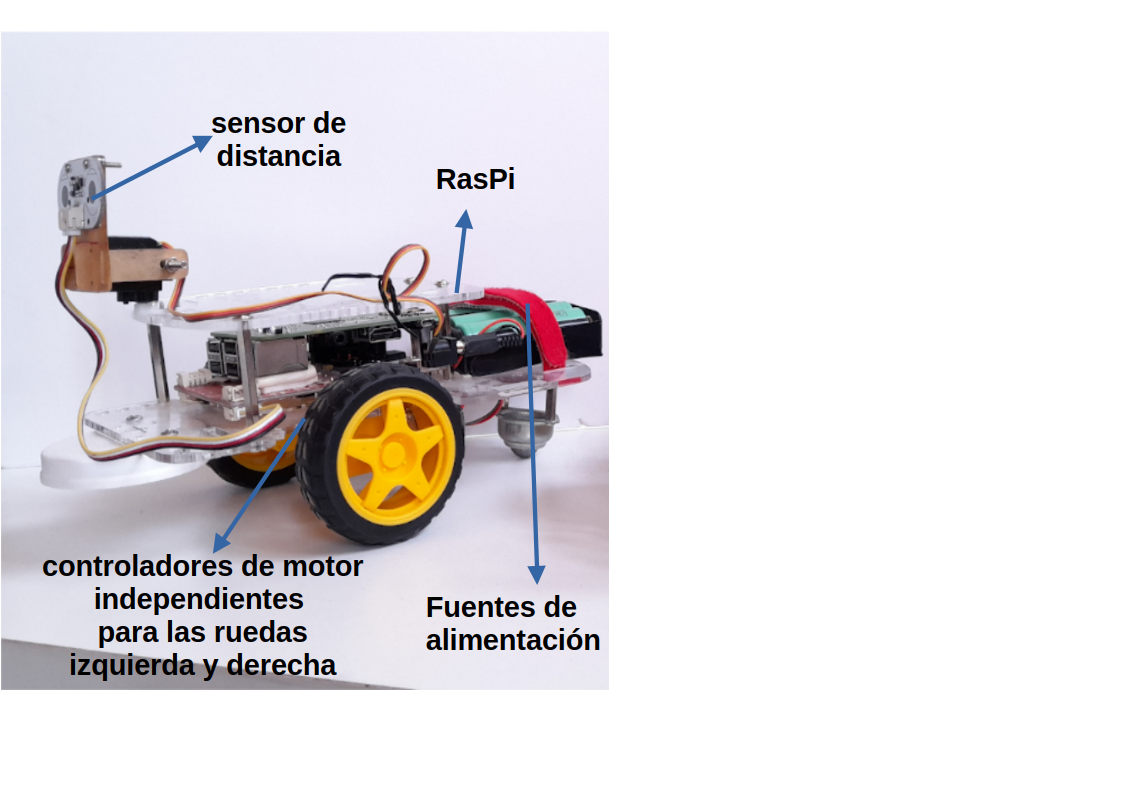
\includegraphics[width=\imsize]{robot_gopigo.png}
	\caption[Esquema del Robot GoPiGo de Dexter Industries, Mostrando Sensores de Distancia, Motores y Raspberry Pi Integrada, Utilizado en Conjunción con la Simulación del Connectoma de C. elegans.  ]{ Esquema del Robot GoPiGo de Dexter Industries, Mostrando Sensores de Distancia, Motores y Raspberry Pi Integrada, Utilizado en Conjunción con la Simulación del Connectoma de C. elegans.}\label{fig:robot}
\end{figure}



\subsection{Simulación de la dinámica neuronal en el connectoma de C. elegans}\label{sec:dinamica}

El robot sigue el diseño propuesto por Busbice, utilizando el connectoma de C. elegans (disponible en \url{https://github.com/openworm/}) para controlar un robot de dos ruedas. Para interactuar con el robot, se han creado dos módulos de Python: un módulo de entrada que lee los sensores del robot y estimula las neuronas apropiadas cuando se alcanzan umbrales específicos, y un módulo de salida que acumula estímulos de las neuronas motoras y, a su vez, envía la cantidad de potencia que se aplicará a cada uno de los dos motores. Estos dos módulos actúan como interfaces entre el robot y el connectoma.


\subsubsection{Modulo de entrada sensorial}

El robot utiliza un sensor de distancia GoPiGo para detectar obstáculos (\url{https://www.dexterindustries.com/store/distance-sensor/}). El sensor de distancia se ubica en la parte frontal del robot y se emplea para medir la distancia a los objetos en el camino del robot. Inicialmente, se utilizó un sensor ultrasónico estándar HC-SR04 para detectar obstáculos, pero se encontraron imprecisiones en las lecturas cuando el robot estaba en movimiento debido a que este tipo de sensor utiliza ondas de sonido para medir la distancia, y estas ondas pueden ser afectadas por el movimiento del robot. Por esta razón, se optó por cambiar al sensor GoPiGo Laser, el cual emplea el método de tiempo de vuelo para medir la distancia. Este método resulta mucho más preciso y no se ve afectado por el movimiento del robot. El proceso de detección de obstáculos funciona de la siguiente manera:


\begin{enumerate}
\item El sensor de distancia emite un pulso láser.
\item El pulso láser rebota en el obstáculo y regresa al sensor de distancia.
\item El sensor de distancia mide el tiempo que tarda el pulso láser en viajar de ida y vuelta.
\item Utilizando el tiempo de viaje, el sensor de distancia calcula la distancia al obstáculo.
\end{enumerate}


El sensor GoPiGo Laser ofrece varias ventajas sobre otros sensores de distancia basados en ultrasonido, incluyendo su precisión, velocidad y alcance. Puede medir la distancia de manera rápida y precisa, lo que lo convierte en una elección idónea para aplicaciones que requieren detección de obstáculos en tiempo real y con un alcance de hasta 5 metros, lo que resulta adecuado para situaciones en las que se necesita detectar obstáculos a distancia. Además de estas ventajas, el sensor GoPiGo Laser es fácil de instalar y usar, ya que se puede conectar a un puerto I2C en la placa Raspberry Pi y se puede utilizar con la biblioteca \textbf{DistanceSensor}. Las instrucciones detalladas sobre cómo conectar el sensor de distancia al robot se encuentran disponibles en \url{https://www.dexterindustries.com/GoPiGo/get-started-with-the-gopigo3-raspberry-pi-robot/}.


Basándonos en resultados de experimentos neurobiológicos y etológicos que demuestran que la nariz de C. elegans es una región altamente sensible, lo que lleva al nematodo a detenerse y cambiar de dirección cuando se encuentra con obstáculos (\Cref{sec:toquenariz}), decidimos utilizar el sensor mencionado para simular el sentido del tacto en la nariz del gusano. El sensor se activa cuando el robot se encuentra a menos de 30 centímetros de un objeto, una distancia que se ha comprobado ser efectiva. Las neuronas sensoriales estimuladas cuando el robot se encuentra a menos de 30 cm de un objeto son las siguientes: ASHL, ASHR, FLPL, FLPR, OLQDL, OLQDR, OLQVL, OLQVR, todas asociadas a este circuito sensorial.


\subsubsection{Detección de comida}

Detección de comida: Cuando el sensor de distancia no detecta obstáculos, estimulamos las neuronas quimiosensoriales responsables de la búsqueda de alimentos. Basándonos en resultados experimentales (\Cref{sec:quimiosensacion}) del comportamiento de búsqueda de alimentos, estimulamos las siguientes neuronas: ADFL, ADFR, ASGL, ASGR, ASIL, ASIR, ASJL, ASJR. En general, la estimulación de las neuronas sensoriales de alimentos activa el connectoma de manera más efectiva y hace que el robot comience a moverse hacia adelante.


 \subsubsection{Modulo de salida motora}
 
 
 Módulo de salida motora: El módulo de salida motora captura las salidas de las neuronas motoras y almacena los valores en una matriz en la que cada celda representa un músculo del cuerpo de C. elegans. Las neuronas motoras se conectan a los músculos para excitarlos o inhibirlos. El circuito neuromotor del gusano utiliza conexiones excitatorias e inhibidoras, lo que permite al gusano moverse de manera ondulante, contrayendo algunos músculos mientras relaja otros y viceversa. En total, hay 95 músculos corporales que recorren todo el cuerpo del gusano: 24 en la parte superior izquierda, 23 en la parte inferior izquierda, 24 en la parte superior derecha y 24 en la parte inferior derecha. Los músculos del cuerpo se dividen en izquierdos y derechos, y el valor acumulado se envía a los motores respectivos del robot. La velocidad máxima del motor se establece en 1000 DPS (grados por segundo), aunque este valor se suele reducir a 150 para evitar movimientos excesivamente rápidos en superficies lisas, aunque puede ajustarse en cualquier momento. Cuando el valor acumulado excede 150, el programa de salida lo restablece a 150. La relación entre los valores acumulados de los músculos izquierdos y derechos determina las señales que se envían a los motores del robot. La \Cref{fig:robot_2} muestra un diagrama de flujo que representa cómo se genera la salida motora.
 

 
  \begin{figure}[h!]
 	\centering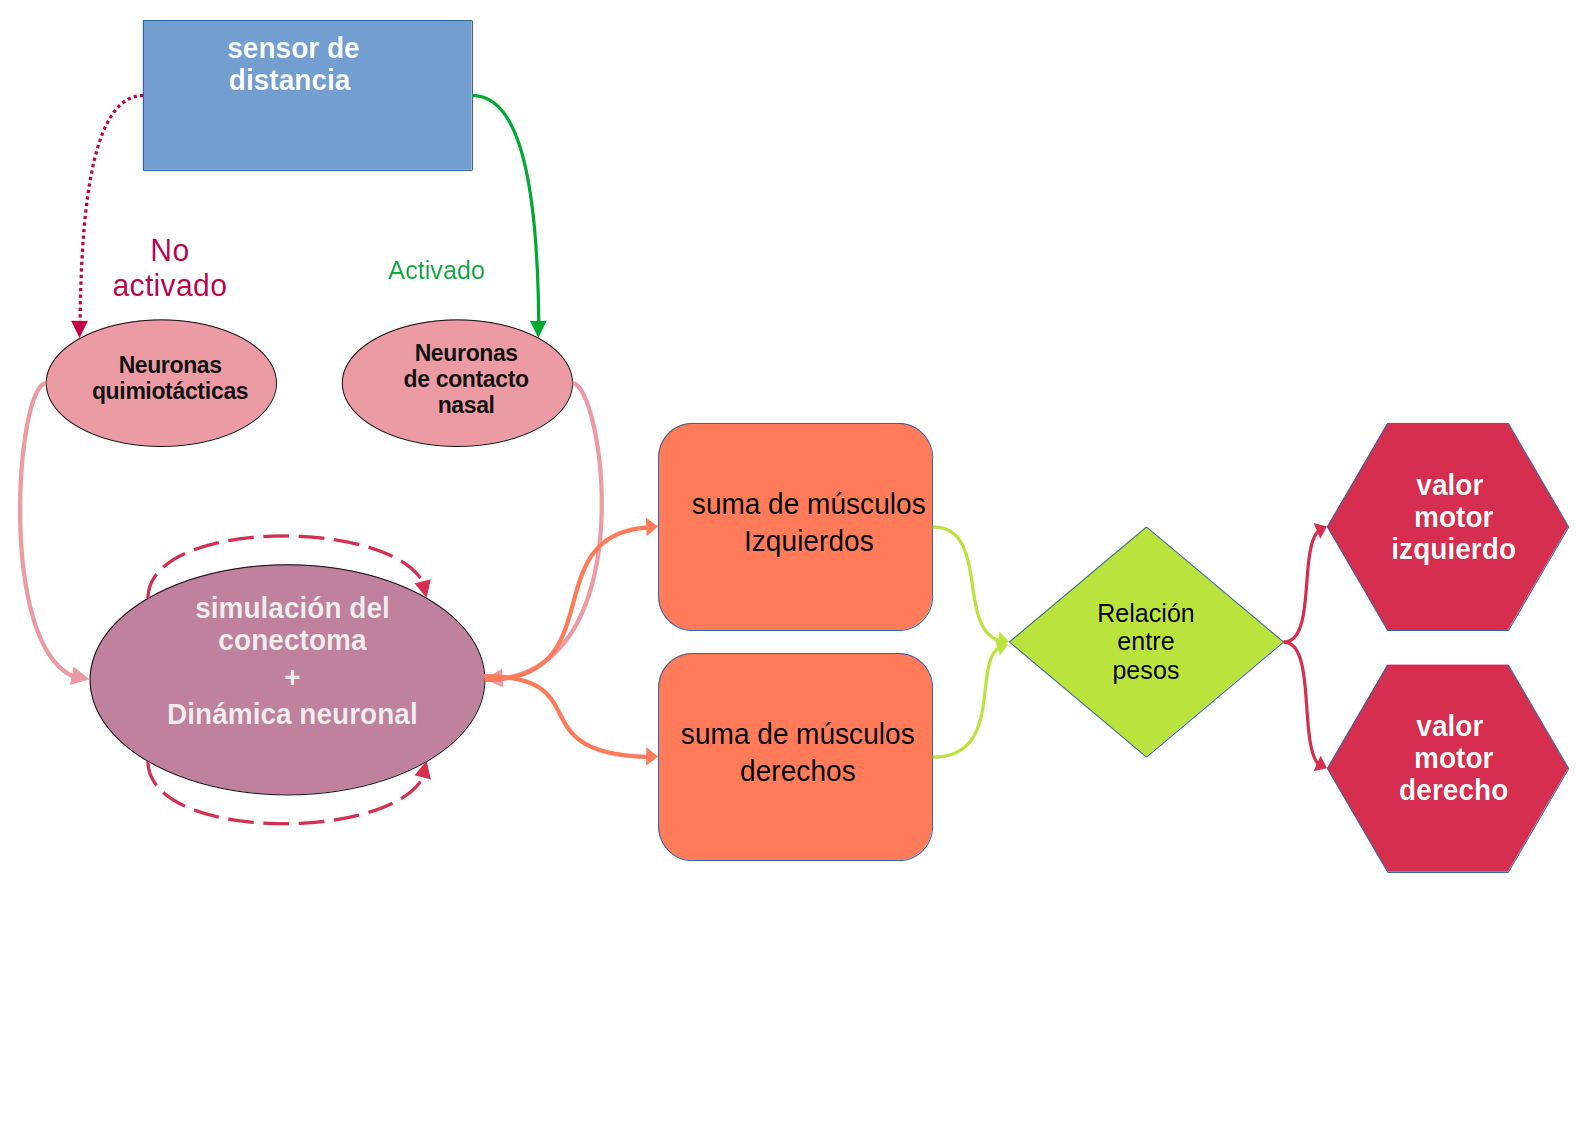
\includegraphics[width=\imsize]{robot_2.png}
 	\caption[Diagrama de Flujo que Ilustra la Generación de la Salida Motora.]{Diagrama de Flujo que Ilustra la Generación de la Salida Motora.}\label{fig:robot_2}
 \end{figure}
 

 
 
  \subsubsection{Modulo del conectoma}
 
El connectoma en sí se compone de un diccionario de Python con 300 entradas, cada una representando una neurona del connectoma de C. elegans (por ejemplo, AVAL, DB02 y VD03). Cada neurona está asociada a un diccionario que contiene las conexiones con otras neuronas, y el número de conexiones se utiliza como valor ponderado. Cuando una neurona dispara, se envía un valor ponderado a las neuronas conectadas. El programa principal se encarga de coordinar la simulación y controlar el robot.


 \subsection{Robot personalizado}

El robot personalizado sigue esencialmente los mismos pasos de construcción que el GoPiGo, pero en lugar de utilizar la placa GoPiGo 2 para el control de motores, emplea un controlador de motor dual L9110S (consulte las \Cref{fig:robot_personalizado,fig:robot_nuestro1,fig:robot_nuestro2}). En las \Cref{fig:sensor_distancia1,fig:sensor_distancia2} se muestra el diagrama de cableado del robot personalizado, que incluye la conexión del sensor de distancia directamente a la Raspberry Pi 3B y el cableado del controlador de motor L9110S.


\begin{figure}[h!]
	\centering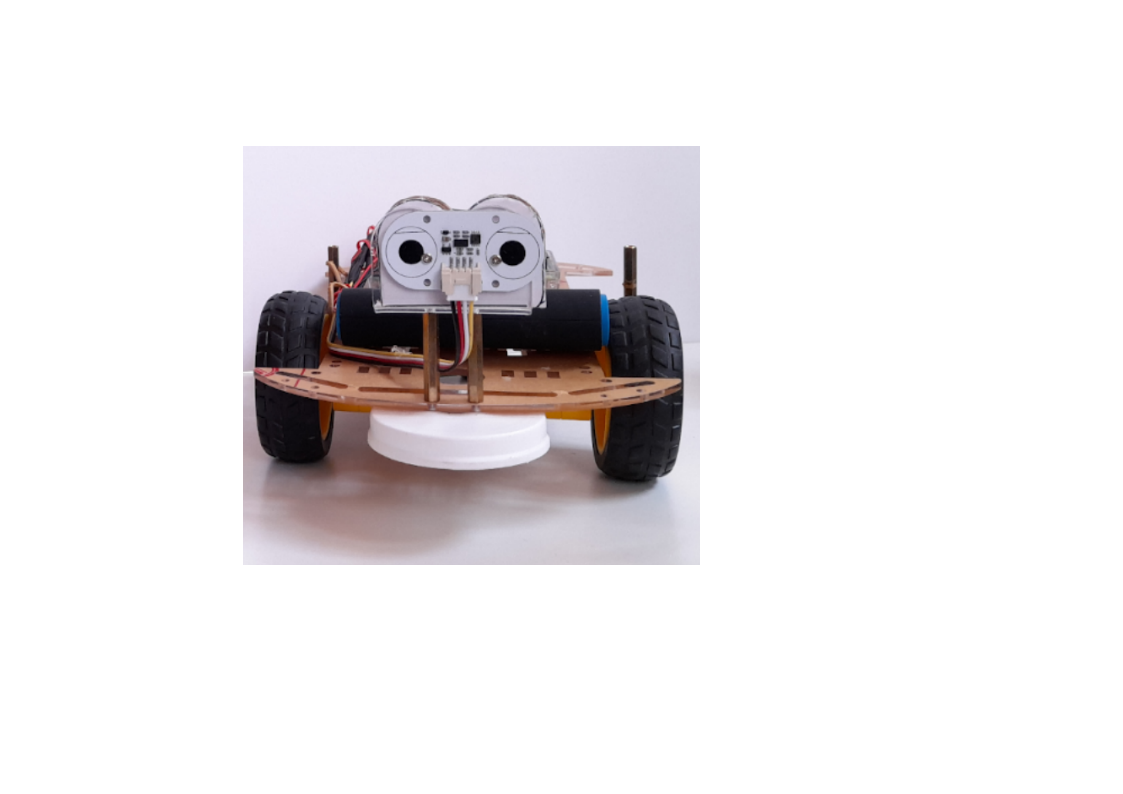
\includegraphics[width=\imsize]{robot_personalizado}
	\caption[Robot Personalizado Empleado en Nuestros Experimentos. ]{ Robot Personalizado Empleado en Nuestros Experimentos. Dado que el hardware del robot GoPiGo no es de código abierto, optamos por construir un robot personalizado, como se muestra a la derecha en la figura. En lugar de la placa GoPiGo 2, utilizamos un controlador de motor dual L9110S para el control de los motores. Este enfoque permite la construcción asequible del robot con componentes de fácil acceso y bajo costo.}\label{fig:robot_personalizado}
\end{figure}


\begin{figure}[h!]
	\centering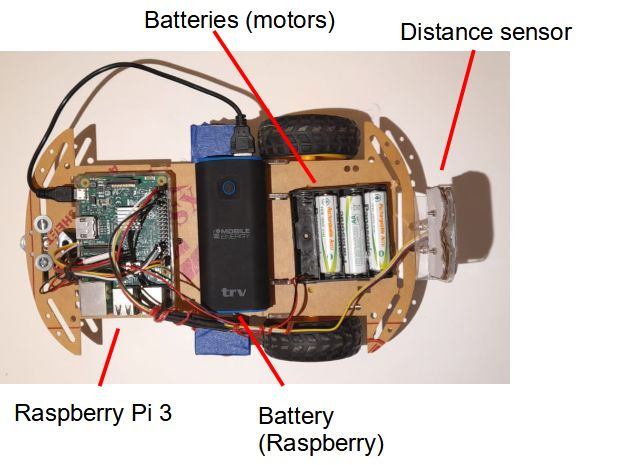
\includegraphics[width=\imsize]{robot_nuestro1.png}
	\caption[Vista Superior del Robot Personalizado.  ]{ Vista Superior del Robot Personalizado. En la imagen, se observa a la izquierda la Raspberry Pi, que ejecuta la simulación numérica para controlar el robot. La caja rectangular negra representa la batería que suministra energía a la Raspberry Pi, mientras que se emplea un paquete de baterías independiente para alimentar los motores. Además, se aprecia un sensor de distancia ubicado en la parte frontal del robot. }\label{fig:robot_nuestro1}
\end{figure}



\begin{figure}[h!]
	\centering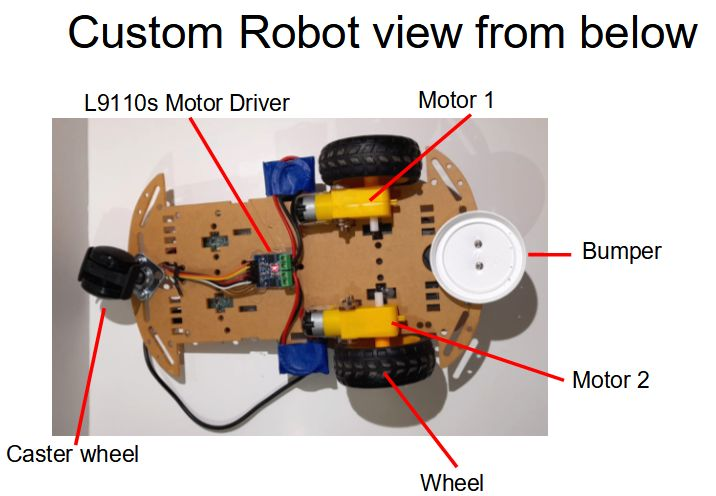
\includegraphics[width=\imsize]{robot_nuestro2.png}
	\caption[ Perspectiva Inferior del Robot Personalizado.]{ Perspectiva Inferior del Robot Personalizado. En esta vista, se aprecia la rueda giratoria a la izquierda, que proporciona soporte y facilita la maniobrabilidad del robot. En la parte inferior se encuentra el pequeño controlador de motores L9110s, permitiendo una conexión directa a los motores (en amarillo) que controlan las ruedas. Para proteger el sensor de distancia de posibles colisiones, se ha adjuntado un parachoques de goma en la parte delantera del vehículo.}\label{fig:robot_nuestro2}
\end{figure}


\begin{figure}[h!]
	\centering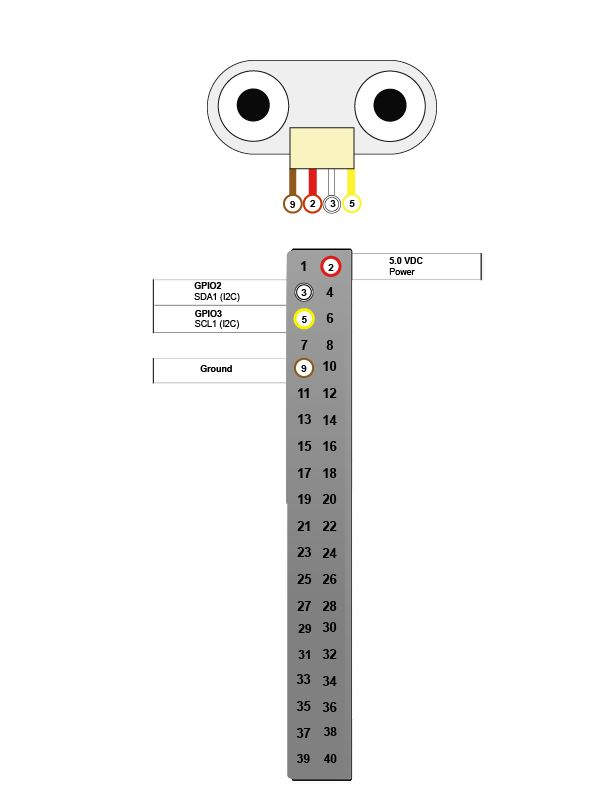
\includegraphics[width=\imsize]{sensor_distancia1.png}
	\caption[Conexión del Sensor de Distancia. ]{Conexión del Sensor de Distancia. En esta representación, se ilustra la conexión del sensor de distancia del GoPiGo directamente a los encabezados GPIO de una Raspberry Pi 3B en el robot personalizado. Las conexiones incluyen: Tierra (Ground), pin 9 (marrón), Alimentación (Power), pin 2 (rojo), SDA1 I2C, pin 3 (GPIO2, blanco) y SCL1 I2C, pin 5 (GPIO3, amarillo).}\label{fig:sensor_distancia1}
\end{figure}


\begin{figure}[h!]
	\centering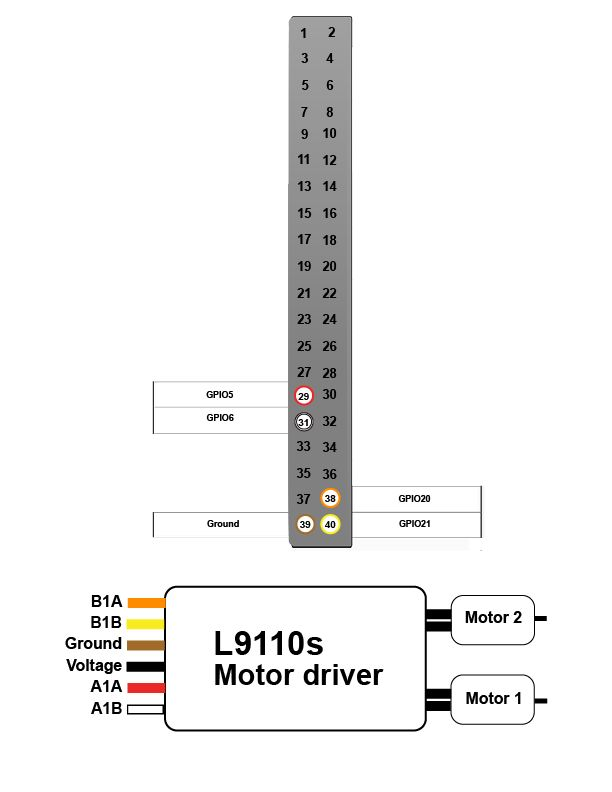
\includegraphics[width=\imsize]{sensor_distancia2.png}
	\caption[Conexión del Controlador de Motor.]{ Conexión del Controlador de Motor. En esta ilustración, se detalla cómo el controlador del motor L9110s se conecta a ambos motores y a los encabezados GPIO de una Raspberry Pi 3B en el robot personalizado. Las conexiones comprenden: B1A, pin 38 (GPIO20, naranja), B1B, pin 40 (GPIO21, amarillo), Tierra, pin 39 (marrón), Voltaje (conexión directa a la batería de 5V, negro), A1A, pin 29 (GPIO5, rojo) y A1B, pin 31 (GPIO6, blanco).}\label{fig:sensor_distancia2}
\end{figure}


\section{Dinámica neuronal global}\label{sec:dinamicakato}

Para explorar la dinámica global del robot que emula la actividad neuronal del C. elegans, hemos seguido la metodología propuesta por Kato et al. \cite{kato_global_2015}. En una primera etapa, calculamos las derivadas temporales de la actividad neuronal del robot. Para lograr esto, empleamos el método de diferenciación regularizada de variación total, cuyos detalles y justificaciones se encuentran en el \Cref{C:ap1}. La regularización desempeña un papel fundamental al reducir el ruido y la variabilidad en los datos, sin comprometer la información crítica.


Posteriormente, aplicamos el Análisis de Componentes Principales (PCA) a las derivadas temporales. Para este propósito, utilizamos la función de \textbf{PCA} de la biblioteca scikit-learn \footnote{https://scikit-learn.org/stable/modules/generated/sklearn.decomposition.PCA.html}. Esta técnica nos permitió no solo obtener los componentes principales (PC) ponderados de las neuronas, sino también calcular la varianza explicada por cada uno de estos componentes. Los PC se derivaron considerando la estructura de covarianza presente en los datos normalizados. Para una comprensión más completa de los PC, se recomienda la lectura de la referencia  \cite{noauthor_principal_2002}.

Con el objetivo de facilitar la interpretación de los resultados, aplicamos un filtro de promedio móvil a las trayectorias en el espacio de fases generadas mediante PCA. Este filtro consistió en un promedio de 10 muestras sucesivas. Paralelamente, generamos una serie de tiempo correspondiente a cada PC, denominada PC temporal. Esta serie se obtuvo mediante un promedio ponderado de las series temporales que abarcaban múltiples neuronas. Los PC temporales capturan señales compartidas por grupos de neuronas, que se agrupan en función de sus correlaciones.


Es importante destacar que realizamos el análisis PCA sobre las derivadas temporales de los datos, ya que los PC resultantes produjeron trayectorias en el espacio de estado que presentaban una organización espacial más coherente. Este enfoque nos brindó una visión más estructurada y representativa de la dinámica global del robot y su relación con el conectoma del C. elegans.



\section{Discusión}

En el marco de nuestra investigación, la elección de este diseño específico de robot se fundamenta en sus características intrínsecamente atractivas. La simplicidad en su construcción y su costo reducido lo destacan como una opción altamente replicable y económicamente eficiente en el contexto de la investigación científica. No obstante, la innovación reside en la simulación neuronal que rige el comportamiento del robot. Dicha simulación se basa en unidades dinámicas elementales e incorpora información biológica derivada del conectoma, lo que confiere al robot la capacidad de manifestar comportamientos emergentes, permitiéndole desenvolverse de manera autónoma y sortear obstáculos de forma natural.

Este modelo presenta una serie de distinciones clave en comparación con la mayoría de las simulaciones:

Primero, se trata de un modelo completo del conectoma, aunque es importante tener en cuenta que no se han incorporado todos los orgánulos o entradas sensoriales en el modelo en la etapa actual. Por ejemplo, los receptores de estiramiento, que podrían desempeñar un papel importante en los comportamientos de locomoción de C. elegans, aún no forman parte de este modelo en su estado actual de desarrollo.

Además, a diferencia de las simulaciones discretas, este modelo sigue una dinámica continua. La estimulación es constante y activa, imitando la operación de un sistema nervioso en tiempo real. Las modificaciones en la información sensorial tienen un impacto directo y continuo en el comportamiento del robot.

La naturaleza física del modelo también es una característica distintiva. El Connectome se encuentra conectado a un robot tridimensional real, lo que posibilita una interacción genuina con su entorno. Esta interacción es altamente impredecible y fundamental para la comprensión del comportamiento emergente.

En lo que respecta a la representación neuronal, cada neurona se modela mediante un programa individual, en analogía con el funcionamiento de las neuronas biológicas. Las entradas dendríticas y las salidas axonales solo responden a la cantidad de estimulación recibida por el programa correspondiente.

Dado que el Conectoma se representa mediante programas individuales, el tiempo de generación de la estimulación no es fijo, sino que varía según la evolución de los factores ambientales. El aspecto temporal es crucial, ya que la estimulación cambia a medida que los factores ambientales se modifican. Cada programa se configura para disparar su axón solo cuando se alcanzan ciertos umbrales, y con el tiempo, el programa se despolariza.

Sin embargo, a pesar de las ventajas mencionadas, hasta el momento no hemos realizado un análisis exhaustivo de la dinámica del modelo ni de su correlación con las acciones del robot. El capítulo siguiente se enfoca en presentar los resultados derivados de la aplicación de este modelo robótico al estudio del comportamiento motor emergente. Además, buscamos, en la medida de lo posible, comparar los resultados obtenidos en el robot con aquellos provenientes de experimentos recientes con C. elegans. Este enfoque nos brinda la oportunidad de adquirir una comprensión más profunda de la capacidad del modelo para simular con precisión el comportamiento del organismo biológico.











